% Klassifiziert den Dokumenten-Typ
% Doku: http://exp1.fkp.physik.tu-darmstadt.de/tuddesign/
% Farben: http://www.tu-darmstadt.de/media/medien_stabsstelle_km/services/medien_cd/das_bild_der_tu_darmstadt.pdf
%  bigchapter: Chapter haben doppelte Schriftgröße
%  linedtoc: Linien im Inhaltsverzeichnis wie bei Überschriften
%  colorbacktitle: Der Dokumenten-Titel wird mir der Accentfarbe hinterlegt
\documentclass[bigchapter,colorback,accentcolor=tud4b,linedtoc,11pt]{tudreport}

% Input Dokument hat das Encoding UTF-8
\usepackage[utf8]{inputenc}
% Wichtiges Paket für Links und verlinktes Inhaltsverzeichnis
\usepackage[ngerman]{hyperref}
% Paket für Fußnoten
\usepackage[stable]{footmisc}
\usepackage{multirow}
\usepackage{colortbl}
% Alternatives package für bilder
\usepackage{wrapfig}
% Paket für amsmath (aligned mathe formeln)
\usepackage{amsmath}
% Farbige tabellen
\usepackage{colortbl}
 
% Paket für Bibliotheks-Verzeichnis, square: Verwende eckige statt runde klammern
% \usepackage[square]{natbib}
% Paket zum Plotten von Datensätzen
\usepackage{pgfplots}
\pgfkeys{%
  /pgfplots/seperators/.style={%
    /pgf/number format/use comma
  },
  /pgfplots/default/.style={%
    /pgf/number format/use comma,
    legend pos=north west,
    x tick label style={/pgf/number format/1000 sep=},
    y tick label style={/pgf/number format/1000 sep=},
    width=0.9\linewidth,
    height=0.40\linewidth,
    scale only axis,
    tick align=outside,
    tickpos=left,
    grid=both,
    tick align=outside,
    minor x tick num=3,
    minor y tick num=4,
    minor grid style={dotted,thin}
  }
}

% Anhänge für Original-Messdaten
\usepackage{fancyvrb}

% Verwende deutsche Bezeichner für Inhaltsverzeichnis, ... (ngerman = New German: neue Rechtschreibung)
\usepackage{ngerman}
% Deutsche Zahlen (entfernt z.B. das Leerzeichen nach einem Dezimal-Komma)
\usepackage{ziffer} 

\usepackage[verbose]{placeins}

%wegen Grafikverschiebung hinzugefügt
\usepackage{float}

%\usepackage{graphicx}
%\usepackage{caption}
\usepackage{subcaption} %Für subfigures

% PDF-Optionen
\hypersetup{%
  pdftitle={TU Darmstadt \- Physikalisches Praktikum für Fortgeschrittene},
  pdfauthor={Esra Bauer, Sören Link},
  pdfsubject={Versuch 2.2-A},
  pdfview=FitH,
}
% Nummeriere formeln in Subsections einzeln
% Kleines makro zur assymetrischen Fehlerangabe

% Entspricht-Zeichen
\usepackage{scalerel}

\newcommand\equalhat{%
\let\savearraystretch\arraystretch
\renewcommand\arraystretch{0.3}
\begin{array}{c}
\stretchto{
    \scalerel*[\widthof{=}]{\wedge}
    {\rule{1ex}{3ex}}%
}{0.5ex}\\ 
=%
\end{array}
\let\arraystretch\savearraystretch
}
%BEGINN TITELSEITE

\title{Interaction of $\gamma$-Radiation with Matter}

\subtitle{Esra Bauer  \\Sören Link}

\subsubtitle{Tutor: Haridas Pai \hfill 4/27/2015}

\author{Esra Bauer, Sören Link, Christian Hoch}

%\settitlepicture{img/title.jpg}

\institution{Physikalisches Praktikum \\für Fortgeschrittene \\ Versuch 2.2-A}

\date{\today}
%ENDE TITELSEITE


\begin{document}
%ANFANG DOKUMENT

%Titelseite einfügen
\maketitle

%Inhaltsverzeichnis einfügen
\tableofcontents

%ANFANG INHALT
\chapter{Introduction}
In this experiment we analyze the radioactive Isotopes $^{22}Na$ and
$^{137}Cs$. This includes determining the convection coefficient $\alpha_K$ of
$^{137}Cs$ and the $\beta^+$ branching coefficient of $^{22}Na$.

\chapter{Theoretical Background}
\section{Radioactice Decay}

Additionally to the well known $\alpha$, $\beta^{\pm}$ and $\gamma$ decay there are two other radioactive decay types which are important for us. First we have electron capture which gives the same progeny as $\beta^+$ decay. The nucleus absorbs an inner atomic electron whereby a proton is converted into a neutron and an electron neutrino. Released energy is given to the neutrino as kinetic energy resp.\ the progeny stays in an excited state if energy is left over. Because the missing electron is replaced by other atomic electrons there is spontaneous X-ray emission.

Second there is the inner conversion as an alternative to $\gamma$ decay. Via direct elektromagnetic interaction energy is transferred from the nucleus to an atomic electron. The nucleus switches into an lower state and the electron is emitted i.e.\ the atom is ionized. As a characteristic number we define the conversion rate as follows

$$\alpha_K = \frac{n_K}{n_{\gamma}}$$

where $n_K$ is the number of emitted conversion electrons and $n_{\gamma}$ is the number of emitted photons.

Below we see the decay schemes of the used Isotopes:

\begin{figure}[H]
    \centering
    \begin{subfigure}[H]{0.44\textwidth}
        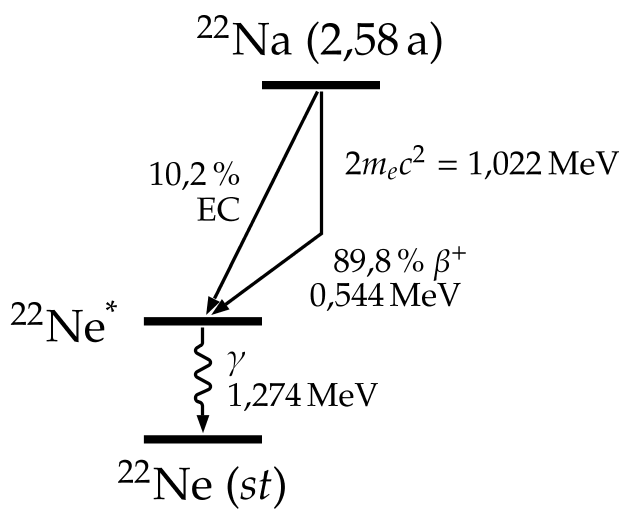
\includegraphics[width=\textwidth]{img/termschema_na22.png}
        \caption{Decay scheme of $^{22}Na$ \cite{na22decay}.}
        \label{fig:gull}
    \end{subfigure}%
    \qquad
    ~%add desired spacing between images, e. g. ~, \quad, \qquad, \hfill etc.
        %(or a blank line to force the subfigure onto a new line)
    \begin{subfigure}[H]{0.44\textwidth}
        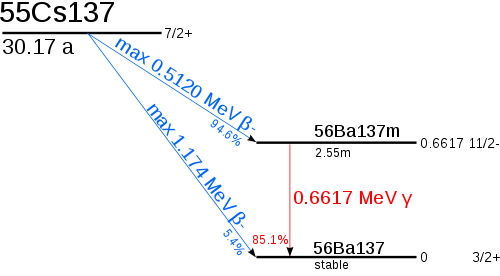
\includegraphics[width=\textwidth]{img/Cs-137-decay.png}
        \caption{Decay scheme of $^{22}Na$ \cite{cs137decay}.}
        \label{fig:tiger}
    \end{subfigure}
    \caption{Decay scheme of the radiactive isotopes used in this experiment.}
\end{figure}

\section{Interaction of $\gamma$-rays with Matter}
The interaction of $\gamma$-rays with matter consists of a superposition
of three different effects. At low photon energies their interaction with matter
is dominated by the photoelectric effect where photons are completely absorbed
by electrons. Bound electrons that absorb a photon in this way are broken free
from their atom, creating an electric current.

Photons with energies in orders of magnitudes ranging from $10^2$ $keV$ to $10^3$ $keV$
mostly interact through elastic scattering with weakly bound electrons. This
results in a transfer of energy from the photon to the electron and is called
the Comtpon effect.

Above energies of $1022keV$ photons traveling in a strong coloumb field can
spontanously convert into an electron and a positron. In doing so the photon
ceases to exists and converts it's energy first into the mass of the $e^-$ and
$e^+$ particle. The remaining energy is then being transferred onto these
particles in the form of kinetic energy. Because the impulse has to be conserved
during this conversion, the effect most often occurs near the nucleus, which can
absorb the impulse of the incident photon. This effect is called pair production
and the likelyhood of it occuring increases with higher photon energies.



\section{Scintillation Spectroscopy}

Because gamma-ray sources produce characteristic spectra with discrete lines it can be used for spectroscopy. We use a scintillation detector which operates as follows. Gamma-rays hit a thallium-doped sodium iodide (NaI) crystal which produces in consequence intense bursts of light. Those flashes unleash electrons at a photocathode which are subsequently multiplied in a photomultiplier tube. This results in an electrical pulse containing meaningful information about the particle that originally hit the detector.

Characteristic numbers for such an detector are the energy resolution and the sensitivity. Energy resolution means the smallest distance between two peaks that can still be identyfied as separate. Due to the high density scintillator its energy resolution is quite good resp.\ better than the resolution of a Geiger-müller counter but not good as that of an semiconductor detector. The sensitivity is defined as the probability for the detection of a particle. Especially in case of inorganic scintillation crystals as used in this experiment, the sensitivity for charged particles is very high due to the use of the phomultiplier tube.

The pulse height spectrum is the distribution of various pulse strenghts (heights) developed while recording the gamma-ray spectrum. The pulse heights are digitized and saved in channels for later spectral analysis.

\chapter{Experimental Setup and Execution}
\begin{figure}[H] 
  \centering
     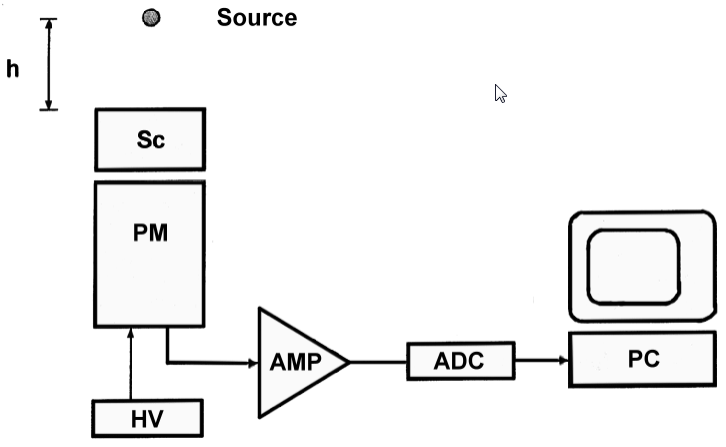
\includegraphics[width=0.8\textwidth]{img/aufbau.png}
     \caption{Experimental setup. As source material we used $^{22}Na$ and
       $^{137}Cs$. In addition we mounted plates of aluminium, cadmium, iron and
     lead behind the source to measure the backscatter radiation. Finally we have
     also measured the background radiation without a radiactive source \cite{Anleitung}.}
  \label{fig:aufbau}
\end{figure}

The experimental setup remains mostly constant throughout the experiment. First
we measured the radioactive spectrum of $^{137}Cs$ with a distance $h$ from the
detecter of $10 cm$. During these measurements
we mounted plates of aluminium, cadmium, iron and lead behind the source to
determine their effect on the spectrum. We've also measured the spectrum of
$^{137}Cs$ through a lead shield.

Afterwards we replaced the caesium isotope with radioactive $^{22}Na$ and
measured it's spectrum twice. The first measurement was done with the natrium
sample mounted $10 cm$ above the scintillation detector. For the second
measurment we put the sample directly on top of the detector.

Each measurement concluded when the main peak of the spectrum reached $3000$ counts.

In the end we measured the background radiation for 31 minutes and 40 seconds.

\chapter{Evaluation}
\section{Analysis of the spectrum of $^{137}Cs$}
\subsection{Energy-calibration}
\begin{center}
\begin{figure}[H]
    \begin{tikzpicture}
    \begin{axis}[
        title={$^{137}Cs$ Spectrum},
        xlabel=channel,
        ylabel=counts,
        height=0.7\textwidth,
        ymin=0,
        xmin=0,
        xmax=320,
        default
    ]
    \addplot[red, only marks, mark=x, mark size=1pt] table[x index=0, y index=1] {data/Cs137-1-no-bg.txt};
    \addlegendentry{$Cs^{137}$ Spectrum}
    \addplot[green, mark=x, mark size=0pt, samples=100, domain=70:110, thick] {1846.49*e^(-0.0367783*(-90.6847+x)^2)};
    \addlegendentry{X-ray peak fit}
    \addplot[blue, mark=x, mark size=0pt, samples=100, domain=190:270, thick] {4549.13*e^(-0.00960132*(-232.427+x)^2)};
    \addlegendentry{Gamma-ray peak fit}
    \end{axis}
    \end{tikzpicture}
    \captionof{figure}{$^{137}Cs$-Spectrum and fits for the x-ray and gamma-peak}
\end{figure}
\end{center}

Using these values we can find the energy calibration for the detector to be $E(c) = 4,44 \cdot c - 369,37$

\subsubsection{Fit Values}
Since radioactive decay and it's detection are stastical processes, we used a
gaussian fit for the detected peaks:

$$f(x) = k\cdot \frac{1}{\sqrt{2 \pi } \cdot \sigma} \cdot e^{-\frac{(x-\mu )^2}{2 \sigma ^2}}$$
\begin{center}
  \begin{tabular}{r|r|r|r|r|r|r}
     Type of peak & $k$     & $\Delta k$ & $\mu$   & $\Delta \mu$ & $\sigma$ & $\Delta \sigma$ \\ \hline
     X-ray        & $17066$ & $597$      & $90,7$  & $0,14$       & $3,69$   & $0,16$          \\ \hline
     Gamma        & $87052$ & $1285$     & $232,4$ & $0,11$       & $7,21$   & $0,14$          \\
	\end{tabular}
\end{center}

\subsection{Energy spectrum}

The calibration explained above gives the following calibrated energy spectrum:

\begin{center}
\begin{figure}[H]
    \begin{tikzpicture}
    \begin{axis}[
        title={$^{137}Cs$ Spectrum},
        xlabel=Energy in keV,
        ylabel=counts,
        height=0.7\textwidth,
        ymin=0,
        xmin=0,
        xmax=1300,
        default
    ]
    \addplot[red, only marks, mark=x, mark size=1pt] table[x index=0, y index=1] {data/Cs137-1-no-bg-calibrated.txt};
    \addlegendentry{calibrated $Cs^{137}$ Spectrum}
    \end{axis}
    \end{tikzpicture}
    \captionof{figure}{}
\end{figure}
\end{center}

Here we see of course the x-ray-peak at 32,9 keV and the photopeak at 661,66 keV because we used them for calibration and also the compton edge, although its difficult to identify. It's located at around 470 keV $\pm$ 25 keV. The theoretical value is determined by
$$E_{Compton} = \frac{E_{\gamma}^2}{2E_{\gamma} + m_ec^2}$$.
That gives 478 keV which means 470 keV matches pretty good. At 170$\pm 25$ keV we can (hardly) see another small peak which is the backscattering peak, its theoretical value is determined by $$E_{backscatter} = E_{\gamma} - E_{Compton}$$
which gives 184 keV.

\subsection{Backscattering peak}

As we can see in the following graph, the height of the backscattering peak depends heavily on the used material: 

\begin{center}
\begin{figure}[H]
    \begin{tikzpicture}
    \begin{axis}[
        title={$^{137}Cs$ Spectrum  with backscatter radiation},
        xlabel=Energy in $keV$,
        ylabel=counts,
        height=0.7\textwidth,
        ymin=0,
        xmin=0,
        xmax=1300,
        default,
        legend pos=north east
    ]
    \addplot[red, only marks, mark=x, mark size=2pt] table[x index=0, y index=1] {data/Cs137-AL-backscattering-no-bg-calibrated.txt};
    \addlegendentry{Aluminium Plate}
    \addplot[green, only marks, mark=x, mark size=2pt] table[x index=0, y index=1] {data/Cs137-Cd-backscattering-no-bg-calibrated.txt};
    \addlegendentry{Cadmium Plate}
    \addplot[blue, only marks, mark=x, mark size=2pt] table[x index=0, y index=1] {data/Cs137-Fe-backscattering-no-bg-calibrated.txt};
    \addlegendentry{Iron Plate}
    \addplot[orange, only marks, mark=x, mark size=2pt] table[x index=0, y index=1] {data/Cs137-Pb-backscattering-no-bg-calibrated.txt};
    \addlegendentry{Lead Plate}
    \end{axis}
    \end{tikzpicture}
    \captionof{figure}{Spectrum of $^{137}Cs$ with 4 different metal covers
      which reflect some of the radiation into the detector via comtpon
      scattering.}
\end{figure}
\end{center}

Generally the backscatter peak has its origin in photons which are backscattered in the shielding around the detector at an angle close to 180$^{\circ}$. That means the photon goes back into the detector and is absorbed i.e. creates the backscatter peak. The probability for compton scattering, which is responsible for backscattering, grows linear with the mass number. Then we have the interaction with the backscattered photons in the detector due to photoeffect because of the relative small energy of the scattered photons. The probability for photoeffect also depends on the mass number, not linear but proportional to Z$^4$. 

\subsection{Absorption by a lead plate}

Here we see the spectra in comparision with/without lead plate:

\begin{center}
\begin{figure}[H]
    \begin{tikzpicture}
    \begin{axis}[
        title={$^{137}Cs$ Spectrum with and without lead shield},
        xlabel=Energy in $keV$,
        ylabel=counts,
        height=0.7\textwidth,
        ymin=0,
        xmin=0,
        xmax=1000,
        default
    ]
    \addplot[red, only marks, mark=x, mark size=2pt] table[x index=0, y index=1] {data/Cs137-1-no-bg-calibrated.txt};
    \addlegendentry{Without lead plate}
    \addplot[blue, only marks, mark=x, mark size=2pt] table[x index=0, y index=1] {data/Cs137-Pb-shield-no-bg-calibrated.txt};
    \addlegendentry{With lead plate}
    \end{axis}
    \end{tikzpicture}
    \captionof{figure}{Effects of a lead shield on the Spectrum of
      $^{137}Cs$. Photons with lower energy get absorbed at a higher rate than
      those with high energies.}
\end{figure}
\end{center}

Obviously the lead plate takes away intensity because of its large mass number, which results in an high absorption of gamma rays (and X-rays, too). Thats also the reason why lead is a suitable material to block gamma-rays off. As you can see the damping is stronger for lower energies which is a result of the different absorption coefficients for photoeffekt and compton scattering. For low energies (photoeffect is dominant) the reduction is proportional to Z$^4$ and for higher energies where compton scattering dominates its proportional to Z. That means for lower energies the higher mass number weakens the gamma-rays more efficiently. If energy grows up further until pair production dominates, reduction becomes more efficient again as its proportional to Z$^2$ then.

\subsection{Conversion coefficient}

The (internal) conversion coefficient describes the rate of internal conversion i.e. its empirically determined by the following formula mentioned before:

$$\alpha_K = \frac{n_K}{n_{\gamma}}$$

Because we cant measure $n_K$ directly we use the following dependency:

$$n_R = \omega_K \cdot n_K$$

where $n_R$ is the number of emitted x-rays and $\omega_K$ is the quantum efficiency. Now we have to determine the source activity which is given by:

$$F = \epsilon \cdot R^{PT} \cdot N \cdot K$$

where N is the number of emitted photons during measurement, F is the area under the total absorption line, $\epsilon$ is the total sensitivity and $R^{PT}$ is the peak-to-total ratio. $\epsilon$ and $R^{PT}$ both depends on the geometry (size of crystal and distance to the source) and the energy of the photons. K is an correction factor.

In case of energies below 100 keV we must consider the absorption at the entry window of the crystal which gives a number for $K_w = 0,85$. Finally we can determine the value of $\alpha_K$ as:

$$\alpha_K = \frac{F_R \epsilon_{\gamma} R_{\gamma}^{PT}  K_{\gamma}}{\omega_K F_{\gamma} \epsilon_R R_K^{PT} K_R}$$

where $K_{\gamma}$  and $K_R$ are related as follows: 

$$K_R = K_{\gamma} - 0,192 \cdot K_w$$.

\section{Analysis of the spectrum of $^{22}Na$}
\subsection{Energy-calibration}
\begin{center}
\begin{figure}[H]
    \begin{tikzpicture}
    \begin{axis}[
        title={$^{22}Na$ Spectrum},
        xlabel=channel,
        ylabel=counts,
        height=0.7\textwidth,
        ymin=0,
        xmin=0,
        xmax=320,
        default
    ]
    \addplot[red, only marks, mark=x, mark size=1pt] table[x index=0, y index=1] {data/Na22-no-bg.txt};
    \addlegendentry{$Na^{22}$ Spectrum}
    \addplot[green, mark=x, mark size=0pt, samples=120, domain=130:160, thick] {5608.36*e^(-0.0450679*(-145.616+x)^2)};
    \addlegendentry{Annihilation peak fit}
    \addplot[blue, mark=x, mark size=0pt, samples=100, domain=210:255, thick] {1002.52*e^(-0.0224958*(-236.12+x)^2)};
    \addlegendentry{Photo-peak fit}
    \addlegendentry{Second peak fit}
    \end{axis}
    \end{tikzpicture}
    \captionof{figure}{$^{22}Na$-Spectrum and fits for the annihilation- and photo-peak}
\end{figure}
\end{center}
For the energy calibration we look at the annihilation peak of $511 keV$ and the
photo peak at $1275 keV$, which we find at channels 146 and 236 respectively.

Using these values we can find the energy calibration for the detector to be $E(c) = 8,442 \cdot c - 738$.

\subsubsection{Fit Values}
Again we used a gaussian fit to characterize the detected peaks:
$$f(x) = k\cdot \frac{1}{\sqrt{2 \pi } \cdot \sigma} \cdot e^{-\frac{(x-\mu )^2}{2 \sigma ^2}}$$

\begin{center}
  \begin{tabular}{r|r|r|r|r|r|r}
     type of peak & $k$     & $\Delta k$ & $\mu$   & $\Delta \mu$ & $\sigma$ & $\Delta \sigma$ \\ \hline
     annihilation & $46825$ & $1119$     & $145,6$ & $0,08$       & $3,33$   & $0,10$          \\ \hline
     photo        & $11847$ & $129$      & $236,1$ & $0,05$       & $4,71$   & $0,06$          \\
	\end{tabular}
\end{center}


\subsection{Energy spectrum}
We have used the annihilation and the photo peak to calibrate the detector and
as such they coincide with literature value. However, the compton peak ranging
from $0 KeV$ to $340,7 keV$ is also clearly visible.
\subsection{Probability of sumpeaks}
A so-called sumpeak occurs whenever two or more incident rays are detected happen in a
shorter time span the temporal resolution of the detector. In such a case the
energies of both incident rays are added together. In our expirment the two
events that can coincide with each other are the detection of annihilation
x-rays and gamma rays. This gives the appearance of an additional peak at their
combined energies of $1786 keV$.

The probability of the occurence of a sumpeak is dependent on the detector and
is quite low in our case. Moving the radioactive source closer to the detecter
increases the frequency at which radioactive events are detected, since the
detector covers a larger angle. This in turn drastically increases the
probability of a sumpeak to occur.
\begin{figure}[H]
\begin{tikzpicture}
\begin{axis}[
  default,
  width=0.48\linewidth,
  title={$^{22}Na$ Spectrum},
  xlabel=channel,
  ylabel=counts,
  height=0.3\linewidth,
  ymin=0,
  xmin=0,
  xmax=2200,
  name=first
]
    \addplot[blue, only marks, mark=x, mark size=1pt] table[x index=0, y index=1] {data/Na22-no-bg-calibrated.txt};
    \addlegendentry{10cm Distance}
    \addplot[red, only marks, mark=x, mark size=1pt] table[x index=0, y index=1] {data/Na22-sum-no-bg-calibrated.txt};
    \addlegendentry{10cm Distance}

As evedient from figure 4.5, there is no sumpeak when the source is 10 cm away
from the detector. However, the increased frequency of incident rays when the
source is placed directly on top of the detector leads to the formation of a sumpeak.

\end{axis}

\begin{axis}[
  default,
  width=0.28\linewidth,
  title={$^{22}Na$ Spectrum at the sum peak},
  xlabel=Energy in $keV$,
  ylabel=counts,
  height=0.3\linewidth,
  ymin=0,
  xmin=1640,
  xmax=1980,
  name=second,
  at=(first.outer south east),
  anchor=outer south west
]
    \addplot[blue, only marks, mark=x, mark size=1pt] table[x index=0, y index=1] {data/Na22-no-bg-calibrated.txt};
    \addplot[red, only marks, mark=x, mark size=1pt] table[x index=0, y index=1] {data/Na22-sum-no-bg-calibrated.txt};
\end{axis}
\end{tikzpicture}
\captionof{figure}{Spectrum of $^{22}Na$ with the source in a 10cm distance from
the detector and directly on top of it. When placed directly on top of the
detector, it registers some radioactive decays as happening simultaneously and
adds the two energies together.}
\end{figure}
\subsection{$\beta^+$-branching ratio}
Analogously to the conversion coefficient of $^{137}Cs$ we can calculate the
$\beta^+$-branching ratio with 
$$\eta = \frac{n_\beta}{n_{tot}} = \frac{\epsilon_{tot} R^{PT}_{tot} K_{tot}
  F_\beta}{\epsilon_\beta R^{PT}_\beta K_\beta F_{tot}}$$


\begin{center}
  \begin{tabular}{r|r|r|r|r|}
     Type of peak & $\epsilon$ & $K$ & $R^{PT}$ & $F$     \\ \hline
     Annihilation & $0,022$    & $2$ & $0,6$    & $46825$ \\ \hline
     Photo        & $0,017$    & $1$ & $0,37$   & $11847$ \\
	\end{tabular}
\end{center}

With our measured data and the values from the experiment room we find that $\eta = 0,94$, whereas the literature value is $\eta = 0,9$.

\subsection{Multiple event process}
To determine the fraction of multiple event processes that count towards the
photo-peak, we first need to get the peak to total ratio: $\eta_{PT}=\frac{n_{tot}}{n_{all}-n\beta}=$


\section{Energy Resolution}

To calculate the Energy Resolution of the detector, we first need the full width
at half maximum (FWHM) of the fitted peaks. The FWHM of a guassian can be
calculated with
$$FWHM = 2 \sqrt{2 \cdot ln2} \cdot \sigma_{e_{\gamma}}$$
where $\sigma_{e_{\gamma}} = \sqrt{E_\gamma}\sqrt{E_{eff}}$. This gives us
$$FWHM = 2 \sqrt{2 \cdot ln2} \cdot \sqrt{E_\gamma}\sqrt{E_{eff}}$$
with $2 \sqrt{2 \cdot ln2} \cdot \sqrt{E_\gamma}$ being the rise of a graph
fitted through $E_\gamma$ (in $keV$) plotted over $\sqrt{E_\gamma}$ (in $\sqrt{keV}$).

\begin{center}
  \begin{tabular}{r|r|r}
    $E_\gamma$ in $keV$ & $\sqrt{E_\gamma}$ in $\sqrt{keV}$ & FWHM in $keV$ \\ \hline
    32,9                & 5,74                              & 38,5          \\ \hline
    511,0               & 22,61                             & 66,2          \\ \hline
    661,7               & 25,73                             & 75,4          \\ \hline
    1275,0              & 35,69                             & 93,7          \\

	\end{tabular}
\end{center}

\begin{center}
\begin{figure}[H]
    \begin{tikzpicture}
    \begin{axis}[
        title={Energy Resolution},
        xlabel=$\sqrt{E_\gamma}$ in $\sqrt{keV}$,
        ylabel=FWHM in keV,
        height=0.7\textwidth,
        ymin=25,
        ymax=100,
        xmin=4,
        xmax=38,
        default
    ]
    \addplot[red, only marks, mark=x, mark size=4pt] table[x=X, y=Y] {data/fwhm.txt};
    \addplot[green, mark=x, mark size=0pt, domain=4:38, samples=10, thick] {27.1052 + 1.84225*x};
    \end{axis}
    \end{tikzpicture}
    \captionof{figure}{Strong quadratic correlation between the FWHM and photon energy}
\end{figure}
\end{center}

Using the rise of the graph $m=1,84$ we calculate $E_{eff}=\frac{m^2}{8ln2}$
to $E_{eff}=0,610 keV$.

\section{Background Radiation}

\begin{center}
\begin{figure}[H]
\begin{tikzpicture}
\begin{axis}[
    title={Background Radiation},
    xlabel=channel,
    ylabel=counts,
    height=0.7\textwidth,
    ymin=0,
    xmin=0,
    xmax=300,
    default
]
\addplot[red, only marks, mark=x, mark size=1pt] table[x index=0, y index=1] {data/background.txt};
\addlegendentry{Background}
\end{axis}
\end{tikzpicture}
\captionof{figure}{}
\end{figure}
\end{center}

The background spectrum shows a visible peak at about $1400keV$ which could be
caused by the decay of $^{238}U$ which emits a photon with an energy of
$1408keV$. The other peaks are too small and diffuse to be clearly identified.


\chapter{Conclusion}

In this experiment we analyzed both general interaction of gamma-rays with
matter like compton scattering, photoeffect etc. and also characteristics of the
isotopes $^{137}Cs$ and $^{22}Na$. With the aid of well known spectral lines we
calibrated the apparatus and could then identify futher lines. Finally we could
determine characteristic numbers as the conversion coefficient and the $\beta^+$
branching ratio. In this way the experiment is a good preparation for gamma-ray
spectroscopy, gamma-ray detection etc.

%ENDE INHALT
\cleardoublepage{}
% Eintrag fürs Inhaltsverzeichnis
\newpage
\begin{thebibliography}{100}
  \bibitem{Anleitung} {Experimental Instructions} \bibitem{na22decay} {Semibyte, homepage of physics lab assistent and qualified
      computer scientist Tobias Krähling:
      \url{http://www.semibyte.de/wp/download/graphicslib/physics/termschema_na22.png}
    [CC BY-NC-SA 3.0]}
  \bibitem{cs137decay} {Wikipedia, the free encyclopedia. By Tubas-en [Public
      domain], via Wikimedia Commons: \url{http://upload.wikimedia.org/wikipedia/commons/thumb/3/3e/Cs-137-decay.svg/500px-Cs-137-decay.svg.png}}
\end{thebibliography}
\end{document}

%%% Local Variables:
%%% mode: latex
%%% TeX-master: t
%%% End:
